\documentclass[12pt]{article}
\usepackage{graphicx} %package to manage images
\graphicspath{ {./figures/} }
\usepackage{caption}
\usepackage[font=scriptsize]{subcaption}
\captionsetup[figure]{labelsep=none}
\captionsetup[table]{labelsep=none}
\usepackage{bbm}
\usepackage{amsmath}
\usepackage{import}
\usepackage{array}
\usepackage{booktabs}     % no extra vertical space between paragraphs
\usepackage{indentfirst}
\usepackage{afterpage}
\usepackage{floatrow}
\usepackage{pdflscape}
\usepackage{soul}
\usepackage{float}
\usepackage{adjustbox}
\usepackage{longtable}
\usepackage{caption}
\usepackage{setspace}
\usepackage{afterpage}
\usepackage[margin=1in]{geometry}
\usepackage[round]{natbib}
\setcitestyle{authoryear}
\usepackage{hyperref}
\usepackage{titlesec}
\usepackage{threeparttable}
\usepackage{setspace}
\usepackage{float}
\floatstyle{plaintop}
\restylefloat{table}
\usepackage{rotating}
\usepackage{authblk}
\usepackage{makecell}


% Optional styling for nicer author/affil typography
\renewcommand\Authfont{\normalsize\bfseries}
\renewcommand\Affilfont{\small\normalfont}
\setlength{\affilsep}{0.3em} % space between author and affiliation

\setlength{\parindent}{0pt}   % standard indent (~0.25 inch)
\setlength{\parskip}{1em}       % no extra vertical space between paragraphs

\titleformat{\section}
  {\normalfont\bfseries\fontsize{14}{16}\selectfont}  % Bold 14pt
  {}{0pt}{}  % No numbering

\titleformat{\subsection}
  {\normalfont\bfseries\fontsize{12}{14}\selectfont}  % Bold 12pt
  {}{0pt}{}  % No numbering

\titleformat{\subsubsection}
  {\normalfont\itshape\fontsize{12}{14}\selectfont}  % Italic 12pt
  {}{0pt}{}  % No numbering
  
\begin{document}

\title{Extended family residence and pregnant women's autonomy and healthcare in India: A Research Note}

\date{\today}

\maketitle
\section{Introduction}


Family relationships play a central role in shaping health and well being. Demographers have investigated the relationships between family structure and relationships among household members, on the one hand, and access to resources, social support, and health outcomes, on the other \citep{lindemann2019family, waite2000family, umberson2010social}. For example, marriage has been found to benefit physical health, psychological well being, and even survival in many contexts \citep{ross1990impact, begashaw2016health, lewis2004conceptualization, soulsby2015marriage, robles2014marital}. Further, research have found that marital quality impacts maternal health through the mechanisms of timely and adequate prenatal care, improved emotional well being during and after pregnancy, and reducing high risk behavior like drinking and smoking during pregnancy (\cite{alipour2019relationship,rosand2011partner}).

India, home to one in six of the world’s births, provides an important context to examine how household structure impacts maternal health.  Although pregnancy occurs almost exclusively within the context of marriage (\citep{banerji2021does}, there is substantial variation in the household structures in which pregnant women reside. Women may live in nuclear households, consisting of only the couple and their children, or they may live in patrilocal extended family households, also called ``joint households.''  Joint households are those in which a woman resides with her husband’s parents, siblings, and other relatives.  Patrilocal joint residence has historically been the normative family structure in India, with land ownership, the responsibility to provide old-age support, and ritual practices organized along male lines \cite{jayachandran2015roots}.  However, a large and modestly increasing fraction of households in India were nuclear -- consisting of a husband, wife, and children -- during the period from 1983 to 2009 \citep{breton2021modernisation}.  A minority of women live in their natal homes, that is, with their own parents, siblings, or relatives.  Their husbands may or may not reside with them.

These family structures shape the social context in which women live, as well as their social status. Newly married women in patrilocal households often occupy the lowest position in both gender and generational hierarchies. Because patrilineal societies are organized along the blood lines of men, daughters-in-law in joint patrilocal households are valued for childbearing and labor, but are ultimately replaceable by other women. Ethnographic and sociological work documents that young daughters-in-law are expected to demonstrate deference to senior family members, take on a disproportionate share of domestic labor, and face restrictions on mobility and decision-making \citep{mandelbaum1988women, jeffery1989labour}. These hierarchies are reinforced in India by limited property rights, low female labor force participation, and inheritance systems that privilege senior male members \cite{jayachandran2015roots}. 

The impact on maternal health of a woman's position as daughter-in-law in an extended-family household can occur through many pathways. Other family members may control spending and not invest adequately in maternal health. Daughters-in-law may have limited ability to take rest or travel for healthcare due to their burden of housework. Daughters-in-law may not get enough to eat when they are pregnant. Mothers facing discrimination and stress in households may develop mental health disorders that affect maternal health. \cite{coffey2022mothers} finds that lower women’s status in patrilocal joint households can be linked to lower survival rates and worse health outcomes for children, likely due to worse nutrition among low-status mothers.

In contrast, in nuclear households married women are less likely to face the same pressures from their in-laws. \cite{desai2008negotiated} finds that many women in India live separately from their migrant husbands, and that a husband's migration increases a woman's autonomy if they live in a nuclear household. That is, if their husband migrates and they live in a joint household, the shift of power due to the absence of their husband goes mostly towards their in-laws. Similarly, \cite{mookerjee2019gender} finds that exogenous shifts from joint to nuclear households increase women’s mobility and participation in decision-making by reducing the control exerted by extended family members.

However, patrilocal households may also offer certain advantages for women, shaping their well-being through multiple mechanisms.  The presence of other adult family members can provide support in the form of shared domestic labor and childcare, which may free up women’s time for other activities \cite{khanna2024role}. Co-residence with extended family members reduces the likelihood of spousal violence \cite{khanna2024role}. Additionally, mothers-in-law and other female household members may be a valuable resource during pregnancy in ensuring that women are getting the care they need \cite{varghese2019coresidence}.  Patrilocal joint households are often characterized by pooled economic resources, inter generational support, and shared domestic labor \citep{wadley1988karimpur}.  

At the same time, hierarchies based on gender and generation may mean that senior family members, particularly mothers-in-law, exercise control over younger women’s mobility and decision making \citep{desai2005women, bloom2001dimensions}. \cite{gupta1999lifeboat} identifies newly married women as the  vulnerable members of the household who are required to demonstrate deference and submission to other family members, and to bear the largest burden of housework. Prior research demonstrates how hierarchies within joint households impact women’s health and that of their children. \cite{coffey2022mothers} find that women married to a younger brother have worse maternal health than women married to an older brother in the same household, and that their children have lower chances of survival and poorer growth.

Nuclear households, in contrast, may provide greater scope for spousal communication and individual autonomy, but may lack the economic and caregiving support available in extended families. Married women in nuclear households are less likely to face the same pressure from their in-laws. The absence of a senior kin may increase women’s participation in household decision making \citep{simkhada2010role,char2010influence}. Further, when husbands in nuclear households migrate for work, women become the head of the household, assuming primary responsibility for  household management, further enhancing her decision making authority \citep{desai2008negotiated}. 

This paper investigates how household structure shapes pregnant women's autonomy and their use of maternal health care.  Our findings cohere with characterizations of nuclear and joint households in the literature: in all of the three survey rounds that we analyze -- from 2005, 2014, and 2021 -- pregnant women in nuclear households have greater decision-making power relative to pregnant women in joint households, but are less likely to use of maternal health care.  We then ask whether and how these relationships have changed in the past two decades.  We find that differences by household type have narrowed, which is consistent with rapid improvement in the accessibility of maternal health care during this period, as well as with important increases in women's decision-making power across household types\citep{ram2026investigation, gandhi2022predictors, muralidharan2017cycling, rai2022use} .

This paper builds upon and dialogs with prior empirical research by \cite{allendorf2013going}, who uses 1992 to 2005 data from India to show that several women's health outcomes were positively associated with joint, rather than nuclear family, residence.  \cite{allendorf2013going}'s paper noted an approximately 8 percentage point increase in the proportion of young women living in nuclear households between 1992 and 2005, and raised the question of how, considering the joint family health advantages that she documented, the shift towards nuclear families might impact women's health in the future.  

In contrast, our research, which specifically focuses on pregnant women, finds that in the last two decades, the trend towards nuclear family residence has reversed.  Pregnant women are 8 percentage points less likely to be living in nuclear households in 2021 than they were in 2005.  Although it is beyond the scope of this research note to investigate reasons for pregnant women's increasing residence in extended families, fertility decline is likely an important factor \footnote{Table \ref{tab:proppatrilocal}) shows the results of a Kitagawa decomposition showing that about half of the increase in nuclear family residence among pregnant women can be explained by the fact that in 2021, pregnant women had fewer prior live births than pregnant women did in 2005.  Lower parity women are more likely to live with their in-laws than higher parity women in both time periods.}. However, one thing that remains consistent with the period \cite{allendorf2013going} studied is that joint families are wealthier than nuclear families, and wealth is a mediator that explains part of the observed gap in maternal health care use between patrilocal and nuclear households. 

This paper contributes to the literature by documenting a reversal in the trend towards nuclear household structure among pregnant women in India. It shows that pregnant women in joint households consistently have lower decision making power than their counterparts in nuclear households, but use maternal healthcare at higher rates. This provides a notable counterexample to the literature which finds or assumes that women's decision making power determines maternal health care use.  In this context, maternal healthcare use is shaped by other factors, such as by economic resources.

\section{Data and Methods}

\subsection{Data} \label{sec:data}

We use data from India’s National Family Health Surveys (NFHS) rounds 3 (2005–2006), 4 (2015–2016), and 5 (2019–2021). The NFHS is India’s Demographic and Health Survey, a nationally representative cross-sectional survey of households and women aged 15–49. These data are publicly available from \texit{www.dhsprogram.com}.

The sample for our primary analysis on trends in household structure and their relationship with autonomy outcomes are those women who are ever married, currently pregnant\footnote{Appendix Table \ref{tab:earlypregnancy} shows that women who report being one or two months pregnant differ systematically from those reporting three or more months of pregnancy. In particular, early pregnancy is more likely to be recognized or reported among more educated and wealthier women. We therefore exclude women reporting one or two months of pregnancy from the analysis.}, and living in either a nuclear or patrilocal household structure. We exclude women living in natal households (about 15 percent of the sample), as this living arrangement represents a substantively different social context from both patrilocal and nuclear households. For example, \cite{dyson1983kinship} explain that closer ties to the natal families indicate higher autonomy for women.\footnote{The prevalence of natal residence among pregnant women is stable across survey rounds, as seen in Appendix figure \ref{fig:bargraph}.  Excluding this group does not affect the interpretation of trends.} For analyses of maternal health care use, instead of focusing on pregnant women, we restrict the sample to ever married women who have given birth in the 3-12 months before the survey.

\subsection{Variables}

\subsubsection{Household structure}
We construct the household structure variable using information on the people residing in the same household as the pregnant woman. We define nuclear households as ones where the woman and her husband are the only two adult members in the household. Patrilocal joint households are defined as the ones where the woman lives with her husband’s adult kin, such as her parent-in-law or adult sibling-in-law. Natal households are those in which the pregnant woman is the daughter or the sister of the household head and none of her husband’s adult kin are present. 

\subsubsection{Sociodemographic variables}  

We define social groups by combining caste and religion, as recommended by the India Human Development Survey (\cite{desai2008india}. Women are classified as Adivasi or Dalit if they report belonging to a Scheduled Tribe or Scheduled Caste, respectively. Muslim women who are not SC/ST are classified as Muslim. Hindu or Sikh women belonging to Other Backward Classes are classified as OBC. Hindu women who are not SC, ST, or OBC are classified as Forward caste. Women who do not fall into these categories (e.g., Christian, Jain, Sikh outside OBC, or no religion) are excluded.\footnote{Only 2.3 percent of pregnant women in NFHS 5 were excluded for this reason.} Uttar Pradesh and Bihar are separated as focus states within regions since they have the highest neonatal mortality in the country (\cite{coffey2025excess}. 

\subsubsection{Outcome variables} \label{sec:outcomes}
To understand women's autonomy during pregnancy, we construct outcomes based on answers to two questions: ``Who usually makes decisions about healthcare for yourself?"  And: ``Who usually makes decisions about visits to your family or relatives?'' We dichotomize these measures by coding women who report that their husband or someone else makes the decision on their behalf as having ‘no say,’ and those who report deciding jointly with their husband or being the only decision maker as ‘some say.’

To measure maternal healthcare use among recently postpartum women, we examine two indicators: birth in a health facility (as opposed to at home) and having 4 or more prenatal visits. The four visit threshold follows the World Health Organization (WHO) and Government of India’s National Health Mission guidelines from 2016.\footnote{In 2016 WHO and NRHM increased the recommended minimum number of visits to 8.  We use 4 because the median pregnant woman in our data was pregnant in 2015.}

\subsubsection{Wealth controls} \label{sec:wealthcontrols}

To capture differences in wealth across household types, we construct a categorical wealth measure based on the full interaction of 8 asset ownership indicators, which has 784 categories. Households are grouped into mutually exclusive categories defined by all combinations of ownership of finished floors, electricity, a radio, a television, a refrigerator, a bicycle, a car, and a latrine or toilet, and these categories are included as fixed effects.


\subsection{Analytical Strategy}
\subsubsection{Patrilocal–nuclear differences and the role of household wealth}

We estimate linear probability models (LPMs) to examine the association between household structure and the four binary outcomes: (1) reporting ``no say'' in decisions about the respondent's own healthcare, (2) reporting ``no say'' in decisions about visits to family or relatives, (3) having an institutional delivery (birth in a health facility), and (4) receiving at least four prenatal visits. We use LPMs because the coefficients can be directly interpreted as percentage point differences, which facilitates comparison across outcomes and survey rounds. In our data, the outcomes are not extremely rare, so linear models provide a reasonable approximation.

For woman $i$ in state $s$, our baseline specification is:

\begin{equation} \label{eq:nocontrols}
Y_{is} = \beta_0 + \beta_1 \text{Patrilocal}_{is} + \mu_s + \epsilon_{is},
\end{equation}

where $i$ indexes women and $s$ indexes states. $Y_{is}$ denotes the outcomes described above, $\text{Patrilocal}_{is}$ is an indicator for residing in a patrilocal joint household (with nuclear households as the reference category), $\mu_s$ are state fixed effects, and $\epsilon_{is}$ is an error term. We estimate this equation separately for each NFHS round: NFHS-3 (2005--06), NFHS-4 (2015--16), and NFHS-5 (2019--21) to examine how the relationships between household structure and the outcomes change over time.

To assess the role of household economic status, we estimate an additional specification that includes $\lambda_{g(i)}$, the wealth group fixed effects described above:

\begin{equation} \label{eq:controls}
Y_{is} = \beta_0 + \beta_1 \text{Patrilocal}_{is} + \lambda_ {g(i)} + \mu_s + \epsilon_{is}.
\end{equation}

In all models, we report standard errors clustered at the primary sampling unit level to account for within-cluster correlation of outcomes.\footnote{All models account for the NFHS complex survey design using sampling weights and stratification.}

\subsubsection{Changes in patrilocal–nuclear differences over time}

To examine how differences between patrilocal extended and nuclear households evolve over time, we estimate models that allow the association between household structure and outcomes to vary across survey rounds. Specifically, for comparisons between 2005-2006 and 2015-2016, as well as 2015-2016 and 2019-2021, we estimate:

\begin{equation} \label{eq:tworounds}
Y_{is} = \alpha + \beta \,\text{Patrilocal}_i + \gamma \,\text{LaterRound}_t
+ \delta \,(\text{Patrilocal}_i \times \text{LaterRound}_t)
+ \lambda_{g(i)} + \mu_s + \varepsilon_{is},
\end{equation}


where $\text{LaterRound}_t$ is an indicator for the later survey round in the comparison. The coefficient of interest $\delta$ captures the change in the patrilocal-nuclear gap between the two survey rounds. As in the main specification, $\lambda_{g(i)}$ denotes wealth-group fixed effects, and $\mu_s$ denotes state fixed effects. This approach allows us to directly test whether the patrilocal–nuclear gap changes across survey rounds, and to assess the statistical significance of these changes.

We also estimate a pooled specification including all three survey rounds to assess changes in the patrilocal-nuclear gap across rounds while using the full sample. The equation is:

\begin{equation} \label{eq:stacked}
\begin{aligned}
Y_{is} = \alpha 
&+ \beta \,\text{Patrilocal}_i
+ \gamma_4 \,\text{NFHS4}_t
+ \gamma_5 \,\text{NFHS5}_t \\
&+ \delta_4 \,(\text{Patrilocal}_i \times \text{NFHS4}_t)
+ \delta_5 \,(\text{Patrilocal}_i \times \text{NFHS5}_t) \\
&+ \lambda_{g(i)} + \mu_s + \varepsilon_{is}.
\end{aligned}
\end{equation}

2005-2006 is the omitted category; NFHS4 refers to 2015-2016, and NFHS5 refers to 2019-2021. $\lambda_{g(i)}$ denotes wealth-group fixed effects, and $\mu_s$ denotes state fixed effects. The reported coefficients $\delta_4$ and $\delta_5$ measure changes in the patrilocal-nuclear gap relative to the gap in 2005-2006.

\section{Results}
\subsection{Trends in Patrilocal Residence}

Table \ref{tab:patrilocal_subgroups} shows that the share of pregnant women living in patrilocal joint households increased from 61 percent in 2005–2006 to 71 percent in 2019–2021. This increase is observed across all major social groups, with particularly large increases among OBC women (14 percentage points), and smaller increases among Adivasi and Muslim women (5 and 7 percentage points, respectively).

Patrilocal residence increased in all regions except the East. In 2019-2021, patrilocal residence is highest in the North and West (79 and 78 percent, respectively), but even areas with comparatively lower baseline levels of patrilocal residence such as Northeast and South showed a noticeable increase in patrilocal residence.  

Patrilocal residence varies sharply by age and parity. Younger women are substantially more likely to live in patrilocal extended households than older women: in 2019–2021, 85 percent of pregnant women aged 15–19 reside in patrilocal households, compared to less than 30 percent among women aged 40–44. Similarly, women with lower parity are more likely to reside in patrilocal households. These patterns are consistent with the view that joint household residence is most common in the early stages of marriage and childbearing. While patrilocal residence declines with age and parity, increases over time are observed across most age and parity groups, except among the oldest women and those with two prior births. 

\subsection{Sample means by household structure}

Table \ref{tab:sumstats} presents summary statistics for autonomy, maternal healthcare use, and wealth outcomes by household structure. Among currently pregnant women, there are large and persistent differences in decision-making power by household type. In 2005–2006, 51 percent of women in patrilocal extended households report having no say in their own healthcare, compared to 32 percent of women in nuclear households. By 2019–2021, these shares decline to 25 and 18 percent, respectively. While autonomy improves substantially over time for both groups, the gap between household types narrows considerably, from 19 percentage points in 2005–2006 to 7 percentage points in 2019–2021. A similar pattern is observed for women’s ability to visit family and friends, where differences of comparable magnitude persist across all survey rounds.

In contrast, maternal healthcare use is higher for women in patrilocal extended households. Among women who gave birth in the 3–12 months preceding the survey, 45 percent of women in patrilocal households delivered in a health facility in 2005–2006, compared to 34 percent in nuclear households. By 2019–2021, although institutional delivery rates increased dramatically for both groups, to 93 percent in patrilocal households and 86 percent in nuclear households, the advantage for patrilocal households remained. A similar pattern is observed for prenatal care: the share of women receiving four or more visits rises from 40 to 61 percent in patrilocal households and from 31 to 53 percent in nuclear households over the same period. Thus, while overall access to maternal healthcare improved substantially, differences by household structure persist.

Patterns in maternal healthcare use mirror differences in household wealth between household structures. Across all survey rounds and for nearly all indicators, women in patrilocal extended households are more likely to live in households with higher asset ownership and better housing conditions. For example, in 2019–2021, 61 percent of pregnant women in patrilocal households live in homes with finished floors compared to 52 percent in nuclear households, and 81 percent have access to a toilet or latrine compared to 71 percent in nuclear households. Ownership of consumer durables such as televisions and refrigerators is also substantially higher in patrilocal households.


\subsection{Patrilocal–nuclear differences and the role of household wealth}

Figure \ref{fig:regresults} presents estimates of the patrilocal coefficient (relative to nuclear households) from equations \ref{eq:nocontrols} and \ref{eq:controls} for each outcome and survey round, with and without wealth controls. These coefficients represent percentage point differences in outcome probabilities between women in patrilocal and nuclear households.

\subsubsection{ Maternal healthcare use outcomes}

In models without wealth controls, women in patrilocal extended households exhibit higher levels of maternal healthcare use across survey rounds. In 2005–2006, women in patrilocal households are 11.3 percentage points more likely to deliver in a health facility than those in nuclear households. This advantage declines over time, to 7.6 percentage points in 2015–2016 and 5.3 percentage points in 2019–2021. A similar pattern is observed for prenatal care: in 2005–2006, patrilocal residence is associated with a 9.0 percentage point higher likelihood of receiving four or more prenatal visits, declining to 5.6 percentage points by 2019–2021.

Controlling for wealth substantially attenuates these differences, indicating that a large share of the advantage in maternal healthcare use among patrilocal households is explained by differences in household economic resources. For institutional delivery, the coefficient declines from 11.3 to 4.5 percentage points in 2005–2006, from 7.6 to 3.6 percentage points in 2015–2016, and from 5.3 to 2.9 percentage points in 2019–2021. In other words, accounting for wealth explains a substantial share—roughly half—of the gap in institutional delivery between patrilocal and nuclear households across survey rounds. For prenatal care, the corresponding reductions are from 9.0 to 2.4 percentage points in 2005–2006, and from 8.2 to 3.9 percentage points in 2015–2016.

\subsubsection{Autonomy outcomes}

In contrast, patrilocal residence is consistently and robustly associated with lower levels of decision-making power. In 2005–2006, women in patrilocal extended households are 16.6 percentage points more likely to report having no say in their own healthcare and 21.1 percentage points more likely to report no say in visits to family and friends. These gaps decline substantially over time but remain non-trivial: by 2019–2021, the corresponding differences are 5.4 percentage points for no say in own healthcare, and 6.5 percentage points for no say in visits to family and friends. 

Controlling for wealth does not attenuate these differences. For both autonomy outcomes, the estimated coefficients remain similar in magnitude with and without wealth controls. This pattern indicates that, unlike maternal healthcare use differences in decision-making power between patrilocal and nuclear households are not explained by differences in household economic resources.

\subsection{Changes in patrilocal–nuclear differences over time}

Table \ref{tab:narrowinggaps} presents estimates of changes in the gap between patrilocal extended and nuclear households over time. Consistent with the descriptive results, differences in women’s autonomy narrow substantially across survey rounds. Between 2005–2006 and 2015–2016, the gap in having no say in healthcare decisions declines by 10.8 percentage points, while the gap in having no say in visiting family and friends declines by 11.6 percentage points. Little additional change occurs between 2015–2016 and 2019–2021 for these autonomy outcomes, but over the full period, the autonomy gaps decline by 13.5 and 17.3 percentage points, respectively.

In contrast, changes in gaps between women in patrilocal and nuclear households for maternal healthcare use outcomes are smaller. For institutional delivery, the gap declines by 2.3 percentage points between 2015–2016 and 2019–2021 and by 4.1 percentage points over the full period. For prenatal care, the gap declines by 2.6 percentage points in the later period, but this change is not large enough to generate a statistically significant decline over the full sample period. Overall, convergence in maternal healthcare use across household structures is more limited than for autonomy. 

Appendix table \ref{tab:decomposition} shows that changes in household structure  composition explains little of the improvement in autonomy and maternal health outcomes with most gains driven by within household type changes. Further in appendix table \ref{tab:proppatrilocal} we observe that declining fertility reflected in first parity pregnancies accounts for a significant portion of the increase in patrilocal residence. Together these results suggests that while improvements in outcomes are not driven by shifts in household composition changes in fertility behavior plays an important role in shaping residence pattern.
 
\section{Discussion}

Using nationally representative data from India (2005-2021) we document a reversal of the earlier trend towards nuclear households. Pregnant women are increasingly residing in joint households, where they have less say in their healthcare and mobility decisions than do pregnant women in nuclear households. However, they  have higher access of maternal health services, including institutional delivery and prenatal care.  This advantage is partly explained by differences in household economic status. In contrast, the disadvantage in autonomy among pregnant women in joint households persists even after controlling for these economic differences.

Decomposition analysis further shows that most of the change over time is driven by within-household type changes rather than shifts in the distribution of women across household structures. This indicates that broader transformations such as improvements in healthcare access, expansion of public health programs and changing social norms are also playing a role in the observed trends. These findings align with existing literature on the role of economic resources in shaping joint family advantages (\cite{allendorf2013going} \cite{breton2021modernisation}). Rather than reflecting an inherent benefit of joint residence the maternal healthcare advantage appears closely tied to the greater material resources of these households alongside evidence that economically less stable couples are more likely to live in nuclear households, reinforcing the observed disparities.

It is important to note that the gap in autonomy between joint and patrilocal households has narrowed over  a 15 year period. This pattern suggests that autonomy may be improving more broadly across society. \cite{pesando2019rethinking} in their review of \cite{goode1963world} theories of family patterns pointed out that the belief that nuclear families are best fitted for industrialized societies was empirically found to be false. Further, they also showed extensive evidence of diverging family patterns across socioeconomic groups within the societies. Thus, the shift might be in tandem with the socio-economic and structural transformation.  But at the same time our findings also indicate that 53 percent (ref: appendix table) of the shift to joint households can be explained by the composition of women at lower parities. This occurs as women move into their husband’s familial home soon after marriage \cite{breton2021modernisation} and are expected to begin childbearing after co-habitation begins \cite{ibarra2020desire}. Declining fertility also further reinforces this pattern by reducing the number of siblings who would be otherwise compete for residence in patrilocal households. Together this suggests that the observed shift towards joint households does not simply reflect a general process of social progress but is also shaped by changing parity composition and demographic constraints on household formation. 

Though material pathways explain maternal healthcare use among women in joint and nuclear households difference in women's autonomy persist between these two household structures. This is an indication of existing hierarchical structure within joint families. Historically, newly married women in joint households occupied the subordinate position within multi-generational families where senior members exercise greater authority. Our findings of persistently lower reported decision making power among women in patrilocal households are consistent with long standing gender and age hierarchy. However, at the same time the decision making power gap for pregnant women between nuclear and joint households have been reducing this can be a result of improvement in quality of relationship between daughter in law and their in-laws which can shape women’s lived experiences within joint families, as positive relational ties are associated with greater perceived autonomy in patrilocal settings \cite{char2010influence}.  

This study has important limitations. Our measures capture utilization but not quality. Four or more prenatal visits do not guarantee adequate, continuous or comprehensive care. Similarly institutional delivery varies across facilities and does not reflect difference in quality of care, mode of delivery or patient experience. Further, measures of autonomy rely on self-reported decision making authority and may not fully capture informal influence or relational dimensions of power within households.  Finally, as NFHS data are cross sectional and measured at the time of the survey, they may not capture the fluid and transitional nature of residence arrangements surrounding marriage and childbirth, as women may move between the different households during this period. This can lead to misclassifications of household structure and obscure how residence shapes autonomy and maternal healthcare outcome.

Together, these findings are consistent with increasing women's empowerment over time but not with a rise in nuclearization. This might be driven by the reduction in overall fertility which might enable more sons to continue living with their parents even after marrying as a result of which there would be less competition for family resources across multiple sons. As we notice despite historically being the less egalitarian option resurgence of joint residence does not uniformly disadvantage pregnant women, nor does it independently explain improvements in maternal healthcare. Rather, household structure appears to be closely linked with broader processes of economic stratification and changing intra household dynamics. Autonomy and healthcare use operate through different pathways, underscoring the need to examine family forms not as fixed categories but as evolving institutional contexts. Understanding how economic resources and relational dynamics intersect within households remains central to explaining contemporary shifts in women’s well-being.






\newpage
\section{Tables and figures}

\begin{table}[!htbp]
    \centering
    \begin{threeparttable}[t]
        \caption{:  Proportion of pregnant women in patrilocal extended households is increasing among all subgroups}
        \label{tab:patrilocal_subgroups}

        \scriptsize
        \setlength{\tabcolsep}{6pt}
        \renewcommand{\arraystretch}{1.3}

        \begin{tabular}{lcccc}
\toprule
 & \multicolumn{1}{c}{NFHS-3} & \multicolumn{1}{c}{NFHS-4} & \multicolumn{1}{c}{NFHS-5} & \multicolumn{1}{c}{\shortstack{Sig.\\(2005--2006 vs.\\2019--2021)}} \\\\
 & \multicolumn{1}{c}{(2005--2006)} & \multicolumn{1}{c}{(2015--2016)} & \multicolumn{1}{c}{(2019--2021)} & \\\\
\midrule
\textbf{All currently pregnant women}&0.59&0.68&0.66&***\\
&&&&\\
\textbf{Social group}&&&&\\
\hspace*{2em}Forward caste&0.45&0.57&0.56&***\\
\hspace*{2em}OBC&0.57&0.65&0.69&***\\
\hspace*{2em}Dalit&0.62&0.73&0.73&***\\
\hspace*{2em}Adivasi&0.69&0.78&0.70&***\\
\hspace*{2em}Muslim&0.56&0.61&0.57&***\\
\hspace*{2em}Sikh/Jain/Christian&0.67&0.76&0.84&\\
&&&&\\
\textbf{Region}&&&&\\
\hspace*{2em}Focus states$^1$&0.61&0.68&0.68&***\\
\hspace*{2em}Central&0.59&0.70&0.72&***\\
\hspace*{2em}East&0.64&0.66&0.60&\\
\hspace*{2em}West&0.65&0.75&0.82&***\\
\hspace*{2em}North&0.68&0.77&0.75&***\\
\hspace*{2em}South&0.58&0.68&0.71&***\\
\hspace*{2em}Northeast&0.49&0.49&0.50&***\\
&&&&\\
\textbf{Age}&&&&\\
\hspace*{2em}15--19&0.76&0.87&0.85&***\\
\hspace*{2em}20--24&0.65&0.75&0.76&***\\
\hspace*{2em}25--29&0.53&0.64&0.62&***\\
\hspace*{2em}30--34&0.41&0.50&0.48&***\\
\hspace*{2em}35--39&0.31&0.32&0.37&***\\
\hspace*{2em}40--44&0.22&0.43&0.24&\\
\hspace*{2em}45--49&0.08&0.17&0.00&\\
&&&&\\
\textbf{Parity (live births)}&&&&\\
\hspace*{2em}0&0.63&0.71&0.66&***\\
\hspace*{2em}1&0.51&0.53&0.54&***\\
\hspace*{2em}2&0.44&0.44&0.43&\\
\hspace*{2em}3+&0.63&0.75&0.75&***\\
&&&&\\
\bottomrule
\end{tabular}


        \begin{tablenotes}
            \item The sample is restricted to women who report being three or more months pregnant at the time of the survey. Women reporting early pregnancy (one to two months) are excluded because early detection is selective.
            \item The sample is further restricted to women in either nuclear or patrilocal extended household structures.
            \item Focus states refer to Uttar Pradesh and Bihar, two Indian states that have a large burden of poor maternal health outcomes.
        \end{tablenotes}
    \end{threeparttable}
\end{table}

\begin{landscape}
\begin{table}[!htbp]
    \centering
    \begin{threeparttable}[t]
        \caption{:  Pregnant women in patrilocal extended households are advantaged in wealth and healthcare utilization, but disadvantaged in autonomy outcomes}
        \label{tab:sumstats}

        \scriptsize
        \setlength{\tabcolsep}{6pt}
        \renewcommand{\arraystretch}{1}
        \label{tab:sumstats}
        \input{tables/table 1 summary stats}

        \begin{tablenotes}
            \item The sample of currently pregnant women includes women who report being three or more months pregnant at the time of the survey. Women reporting early pregnancy (one to two months) are excluded because early detection is selective.
        \end{tablenotes}
    \end{threeparttable}
\end{table}
\end{landscape}



\begin{landscape}
\begin{figure}[H]
    \centering
    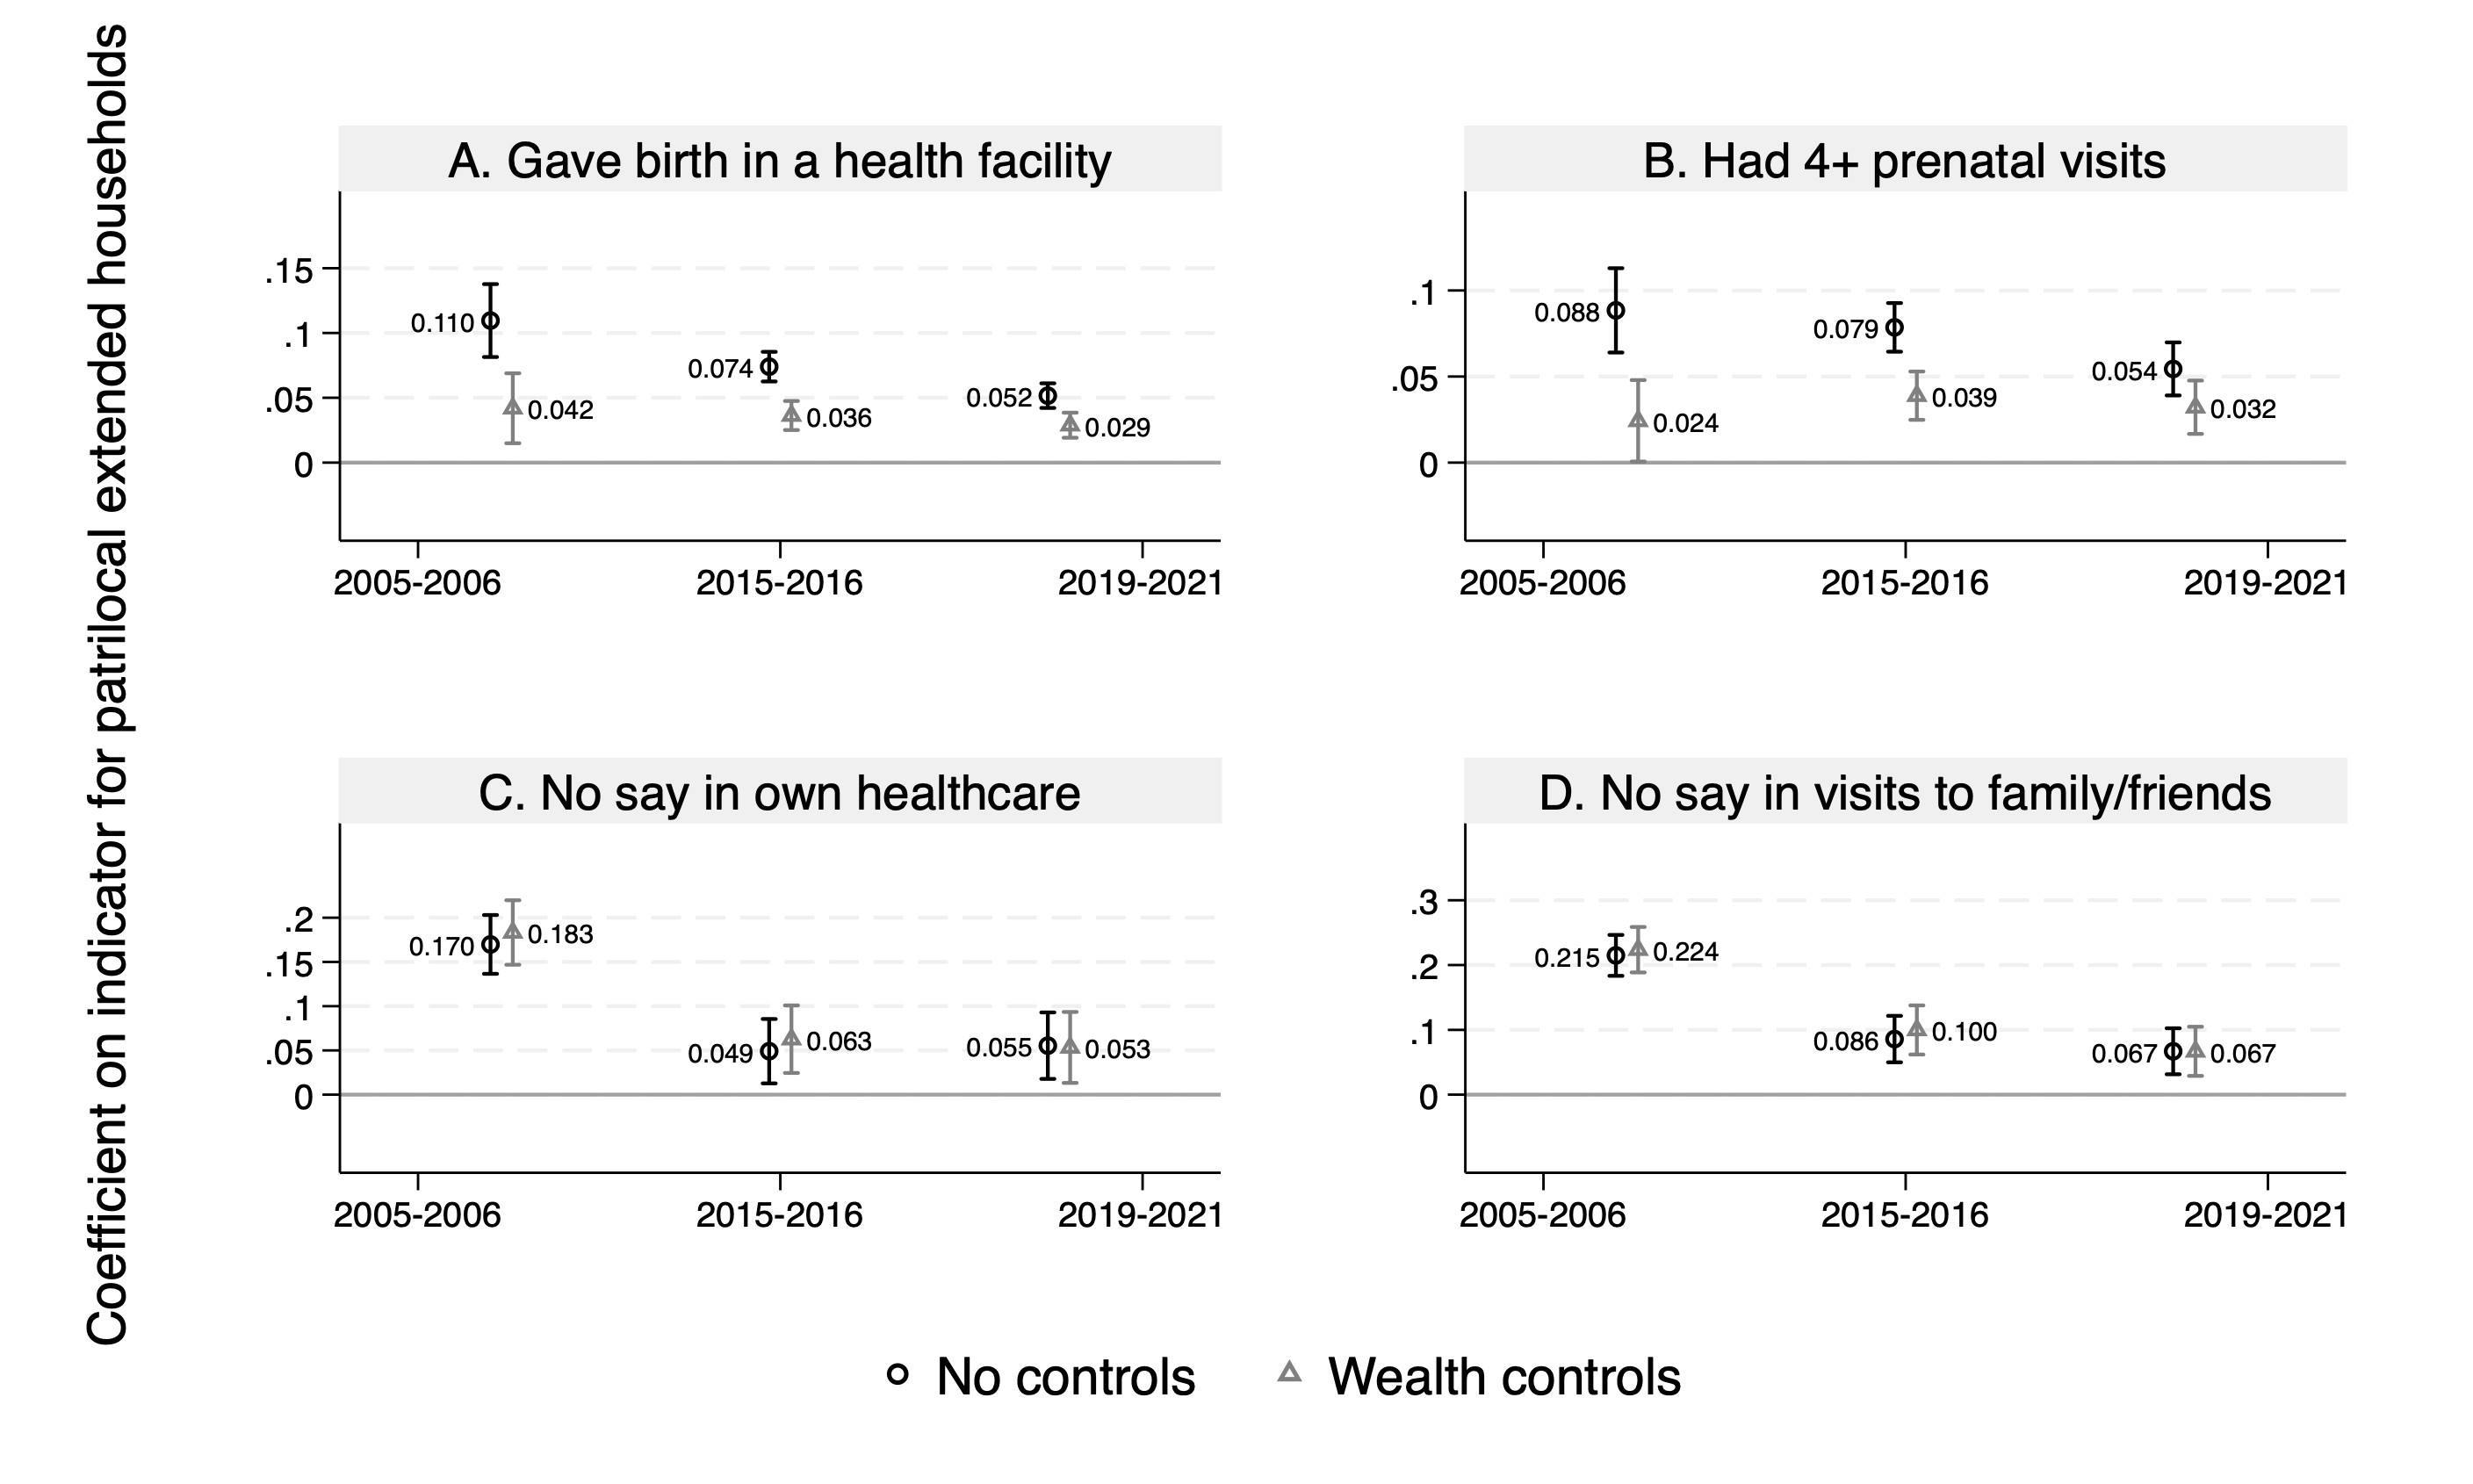
\includegraphics[width=0.85\textwidth] 
    {figures/figure 1 regression coefficients with and without controls.png}
    \caption{: Estimated differences in autonomy and healthcare utilization outcomes for women living in patrilocal extended households relative to nuclear households}
    \label{fig:regresults}
    \parbox{1\linewidth}{\footnotesize Points represent the coefficient on the patrilocal household indicator from linear probability models shown in equations \ref{eq:nocontrols} and \ref{eq:controls}. Panels for outcomes "Gave birth in a health facility" and "Had 4+ antenatal care visits" use the sample of women who gave birth 3-12 months before the survey. Panels for outcomes "No say in own healthcare" and "No say in visits to family/friends" use the sample of women who report being three or more months pregnant at the time of the survey.}
\end{figure}


\end{landscape}


\begin{table}[!htbp]
    \centering
    \begin{threeparttable}[t]
        \caption{: The gap between patrilocal extended and nuclear households in women's autonomy and health care use in narrowing across survey rounds}
        \label{tab:narrowinggaps}

        \scriptsize
        \setlength{\tabcolsep}{6pt}
        \renewcommand{\arraystretch}{1.6}

        \begin{tabular}{lcccc}
\toprule
 & \multicolumn{1}{c}{\shortstack{$\delta$ (Eq.~\ref{eq:tworounds})\\2005--2006 vs.\\2015--2016}} & \multicolumn{1}{c}{\shortstack{$\delta$ (Eq.~\ref{eq:tworounds})\\2015--2016 vs.\\2019--2021}} & \multicolumn{1}{c}{\shortstack{$\delta_4$ (Eq.~\ref{eq:stacked})\\2005--2006 vs.\\2015--2016}} & \multicolumn{1}{c}{\shortstack{$\delta_5$ (Eq.~\ref{eq:stacked})\\2005--2006 vs.\\2019--2021}} \\\\
\midrule
No say in visits to family/friends$^1$&-0.127***&-0.012&-0.127***&-0.177***\\
Gave birth in a health facility$^2$&-0.059*&0.030&-0.054*&-0.043\\
No say in own healthcare$^1$&-0.074***&0.004&-0.077***&-0.107***\\
Had 4+ prenatal visits$^2$&0.001&0.046&-0.006&0.020\\
&(0.031)&(0.034)&(0.031)&(0.033)\\
&(0.021)&(0.022)&(0.021)&(0.020)\\
&(0.033)&(0.041)&(0.032)&(0.037)\\
&(0.021)&(0.021)&(0.020)&(0.020)\\
&N = 12,994&N = 10,832&N = 17,761&N = 17,761\\
&N = 4,708&N = 3,605&N = 6,185&N = 6,185\\
&N = 4,709&N = 3,606&N = 6,186&N = 6,186\\
&N = 12,994&N = 10,832&N = 17,761&N = 17,761\\
\bottomrule
\end{tabular}



    \end{threeparttable}
\end{table}




\newpage
\bibliographystyle{apalike}
\bibliography{references}

\newpage
\section{Appendix}

\appendix

\setcounter{equation}{0}
\renewcommand{\theequation}{A\arabic{equation}}

% Reset and format appendix numbering
\setcounter{section}{-1}
\renewcommand{\thesection}{S.\arabic{section}}
\renewcommand{\thesubsection}{S.\arabic{section}.\arabic{subsection}}

% Make tables/figures labeled A.1, A.2, etc.
\setcounter{table}{0}
\renewcommand{\thetable}{A\arabic{table}}
\setcounter{figure}{0}
\renewcommand{\thefigure}{A\arabic{figure}}

\setcounter{subsection}{0}
\renewcommand{\thesubsection}{A.\arabic{subsection}}

\titleformat{\subsection}
  {\normalfont\bfseries\fontsize{12}{14}\selectfont}
  {\thesubsection}{1em}{}

\titleformat{\subsubsection}
  {\normalfont\itshape\fontsize{12}{14}\selectfont}
  {\thesubsubsection}{1em}{}
    
\subsection{Justification of decision to drop women reporting 1 or 2 months of 
pregnancy}

The main sample of pregnant women used in the paper excludes those who report being 1 or 2 months pregnant at the time of the survey, 
to avoid biasing the results due to selection into early detection and reporting of pregnancy.

To confirm that this the sample of women who report being 1 or 2 months pregnant is systematically different than those reporting 3 or more months of pregnancy, we estimate the following regression on the entire sample of women who report being currently pregnant:

\begin{equation}
Y_i=\beta X_i+\epsilon_i
\end{equation}

where for woman $i$, 
\begin{itemize}
    \item $Y_i$ is an indicator for reporting 1 or 2 months of pregnancy (as opposed to 3 or more)
    \item $X_i$ is a set of indicators for less than primary education, rural residence, whether the woman does not have any sons, 4 age bins, 10 parity and time since last birth categories, and wealth quartiles. 
\end{itemize}

We report the estimated coefficients $\beta$ in table \ref{tab:earlypregnancy} to check the balance of variables in $X_i$ across women reporting 1 or 2 months of pregnancy and women reporting 3 or more.

\begin{table}[H]
    \centering
    \begin{threeparttable}[t]
        \caption{:  Predicting early pregnancy}

        \label{tab:earlypregnancy}
        \scriptsize
        \setlength{\tabcolsep}{10pt}
        \renewcommand{\arraystretch}{1}

        \input{tables/tableA1_predicting_first_quarter_pregnancy1}

        \begin{tablenotes}
            \item Gestational duration is defined for women who report being pregnant at the time of the survey using the reported number of months since the start of the woman's last menstrual period.  If that was not reported for a woman, we her answer to the question, ``How many months pregnant are you?'' to measure gestational duration instead. This substitution is made for 5\% of the women who report being currently pregnant. 
            \item The sample is restricted to women residing in either nuclear or patrilocal extended household structures. 
            
        \end{tablenotes}
    \end{threeparttable}
\end{table}

\subsection{Kitagawa decomposition of changes in family structure}

We use Kitagawa decomposition \citep{kitagawa1955components} to assess whether the increase in the proportion of women living in patrilocal joint households observed between 2005-2006 and 2019-2021 in Table \ref{tab:patrilocal_subgroups} can be explained by compositional shifts in parity. 

For the proportion of women living in patrilocal joint households, $Y$, the change between NFHS-3 (2005-2006) and NFHS-5 (2019-2021) can be written as:

\begin{equation}
\Delta \equiv \bar Y^{5} - \bar Y^{3}
= \Delta_{\text{explained}} + \Delta_{\text{unexplained}}
\end{equation}

\begin{equation}
\Delta_{\text{explained}} =
\sum_{p \in \{1,2,3,4+\}} \big(s_p^{5} - s_p^{3}\big)\frac{Y_p^{5} + Y_p^{3}}{2}
\end{equation}

\begin{equation}
\Delta_{\text{unexplained}} =
\sum_{p \in \{1,2,3,4+\}} \big(Y_p^{5} - Y_p^{3}\big)\frac{s_p^{5} + s_p^{3}}{2}
\end{equation}

\begin{itemize}
    \item where $p \in \{1,2,3,4+\}$ indexes parity
    \item $\bar Y^{3}$ and $\bar Y^{5}$ are the proportion of pregnant women in patrilocal joint households in NFHS-3 (2005-2006) and NFHS-5 (2019-2021)
    \item $Y_p^{3}$ and $Y_p^{5}$ are the proportion of pregnant women in patrilocal joint households within parity $p$ in NFHS-3 (2005-2006) and NFHS-5 (2019-2021)
    \item $s_j^{3}$ and $s_j^{5}$ are the shares of pregnant women at parity $p$ in NFHS-3 (2005-2006) and NFHS-5 (2019-2021)
\end{itemize}

\begin{landscape}

\begin{table}[H]
    \centering
    \begin{threeparttable}[t]
        \caption{: More than half of the increase in patrilocal joint household residence among pregnant women between 2005-2006 and 2019-2021 can be explained by lower parities in 2019-2021}
        \label{tab:proppatrilocal}

        \scriptsize
        \setlength{\tabcolsep}{6pt}
        \renewcommand{\arraystretch}{1.3}

        \input{tables/table A1 household structure decomposition}

        \begin{tablenotes}
            \item Parity refers to the number of prior live births at the time of the interview.  The current pregnancy is therefore not counted.
            \item The sample is restricted to women who report being three or more months pregnant at the time of the survey. Women reporting early pregnancy (one to two months) are excluded because early detection is selective, as shown in table \ref{tab:earlypregnancy}
            \item The sample is also restricted to women residing in either nuclear or patrilocal extended household structures. 
        \end{tablenotes}
    \end{threeparttable}
\end{table}

\end{landscape}



    
\subsection{Distribution of women by household type in NFHS-2005, 2015, and 2021}

The sample used for the main analysis in this paper focuses on pregnant women who live in either nuclear or patrilocal joint household structures, excluding women living in natal households.

Figure \ref{fig:bargraph} shows the composition of household structure in different samples of women. While the main analysis in the paper focuses on pregnant women, trends of increasing joint patrilocal residence are also present in the sample of all women, nonpregnant women, and the sample used in \cite{allendorf2013going}. 

In all samples shown in Figure \ref{fig:bargraph} except the sample used in \cite{allendorf2013going}, the bar graph keeps the subsample of women in natal households to show that its proportion remains stable over time, and that its exclusion does not affect trends in nuclear and patrilocal joint household structures.

\begin{landscape}
    

\begin{figure}[H]
    \centering
    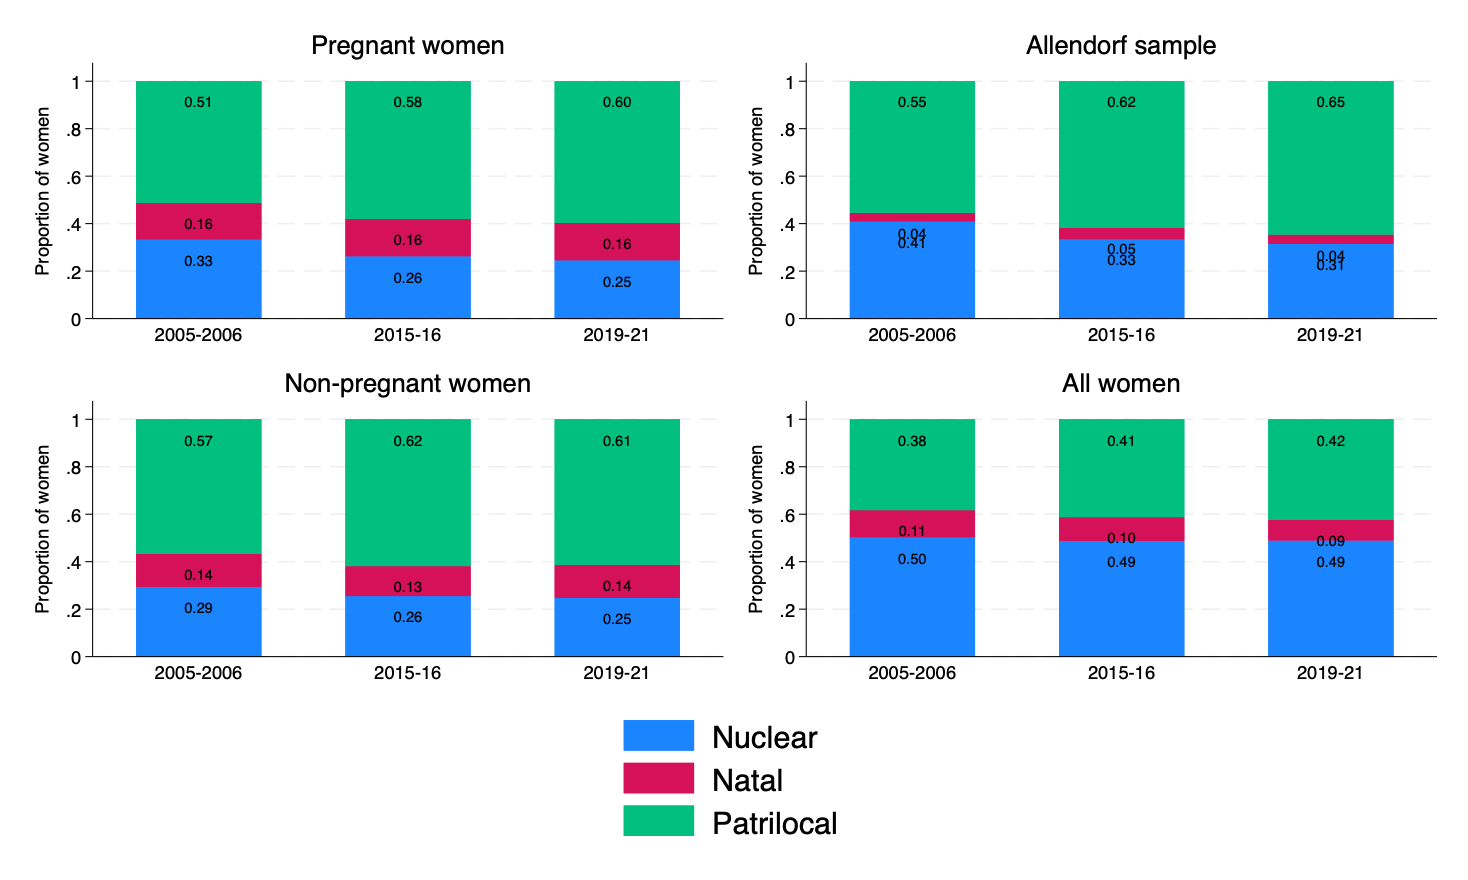
\includegraphics[width=\textwidth] 
    {figures/apdx bar graph four panel.png}
    \caption{: The proportion who reside in natal households remains similar over time in relevant sub-samples of women}
    \label{fig:bargraph}
    \parbox{1\linewidth}{\footnotesize The sample used in \cite{allendorf2012women} includes women who are currently married, living with their husband, between the ages of 15 and 29, usual residents of their household, and living in either nuclear or patrilocal joint household structures.}
\end{figure}

\end{landscape}


\subsection{Kitagawa decomposition of changes in autonomy and health care indicators}


To assess whether changes in autonomy and maternal healthcare are driven by shifts in the distribution of household structure or by changes within household types, we implement a Kitagawa decomposition \citep{kitagawa1955components} comparing NFHS-3 (2005--06) and NFHS-5 (2019--21), using NFHS-3 as the baseline.

For each outcome $Y$, the change between NFHS-3 and NFHS-5 can be written as:

\begin{equation}
\Delta \equiv \bar Y^{5} - \bar Y^{3}
= \Delta_{\text{explained}} + \Delta_{\text{unexplained}}
\end{equation}

\begin{equation}
\Delta_{\text{explained}} =
\sum_{j \in \{N,P\}} \big(p_j^{5} - p_j^{3}\big)\frac{Y_j^{5} + Y_j^{3}}{2}
\end{equation}

\begin{equation}
\Delta_{\text{unexplained}} =
\sum_{j \in \{N,P\}} \big(Y_j^{5} - Y_j^{3}\big)\frac{p_j^{5} + p_j^{3}}{2}
\end{equation}

\begin{itemize}
    \item $j \in \{N,P\}$ indexes household type: nuclear ($N$) and patrilocal ($P$)
    \item $\bar Y^{3}$ and $\bar Y^{5}$ are the mean outcomes in NFHS-3 and NFHS-5
    \item $Y_j^{3}$ and $Y_j^{5}$ are the mean outcomes within household type $j$ in NFHS-3 and NFHS-5
    \item $p_j^{3}$ and $p_j^{5}$ are the proportions of women residing in household type $j$ in NFHS-3 and NFHS-5
\end{itemize}




\begin{table}[H]
    \centering
    \begin{threeparttable}[t]
        \caption{:  None of the improvement in the outcomes is explained by changing composition in household structures}
        \label{tab:decomposition}

        \scriptsize
        \setlength{\tabcolsep}{10pt}
        \renewcommand{\arraystretch}{2.5}

        \begin{tabular}{lccc}
\toprule
Outcome & \makecell{Total change\\(pp)} & \makecell{Share explained by \\household structure (\%)} & \makecell{Share from within-\\household structure changes (\%)} \\
\midrule
No say in own healthcare$^1$&-23.35&-1.72&101.72\\
No say in visits to family/friends$^1$&-28.27&-1.75&101.75\\
Four or more prenatal visits$^2$&22.24&1.15&98.85\\
Birth in a health facility$^2$&50.26&0.54&99.46\\
\bottomrule
\end{tabular}


        \begin{tablenotes}
           \item The sample is restricted to women who report being three or more months pregnant at the time of the survey. Women reporting early pregnancy (one to two months) are excluded because early detection is selective.
            \item The sample is also restricted to women residing in either nuclear or patrilocal extended household structures. 
            
        \end{tablenotes}
    \end{threeparttable}
\end{table}


    



% \begin{landscape}


% \begin{figure}[H]
%     \centering
%     \includegraphics[width=0.85\textwidth] 
%     {figures/figure 1 regression coefficients without state fes.png.png}
%     \caption{: (without state fe) Estimated differences in autonomy and healthcare utilization outcomes for women living in patrilocal extended households relative to nuclear households}
%     \label{fig:regresultsnocontrols}
%     \parbox{1\linewidth}{\footnotesize Same as figure \ref{fig:regresults} but without state fixed effects. Points represent the coefficient on the patrilocal household indicator from linear probability models shown in equations \ref{eq:nocontrols} and \ref{eq:controls}. Panels for outcomes "Gave birth in a health facility" and "Had 4+ antenatal care visits" use the sample of women who gave birth 3-12 months before the survey. Panels for outcomes "No say in own healthcare" and "No say in visits to family/friends" use the sample of women who report being three or more months pregnant at the time of the survey.}
% \end{figure}

% \end{landscape}




% \begin{table}[!htbp]
%     \centering
%     \begin{threeparttable}[t]
%         \caption{: Association between nuclear houshold with patrilocal households with and without wealth controls}
%         \label{tab:proppatrilocal}

%         \scriptsize
%         \setlength{\tabcolsep}{6pt}
%         \renewcommand{\arraystretch}{1.3}

%         \input{tables/table 2 regressions}

%         \begin{tablenotes}
%             \item put table notes here
%         \end{tablenotes}
%     \end{threeparttable}
% \end{table}




%% OLD figures
% \begin{figure}[H]
%     \centering
%     \includegraphics[width=\textwidth] 
%     {figures/figure 1 change in hhstructure.png}
%     \caption{: 1 panel figure showing change showing household structure}
%     \label{fig:ihds_eat_last}
%     \parbox{1\linewidth}{\footnotesize figure notes go here}
% \end{figure}

% \begin{landscape}
    

% \begin{figure}[H]
%     \centering
%     \includegraphics[width=\textwidth]
%     {figures/figure 2 four panel.pdf}
%     \caption{: 4 panel figure showing changes over time in say in own healthcare, say in visits to family, friends, facility birth, and 4+ prenatal visits}
%     \label{fig:ihds_eat_last}
%     \parbox{1\linewidth}{\footnotesize figure notes go here}
% \end{figure}

% \end{landscape}


% \begin{landscape}
    


% \begin{table}[!htbp]
%     \centering
%     \begin{threeparttable}[t]
%         \caption{:  patrilocal coefficient in different regression specifications}
%         \label{tab:reg_coefs}

%         \scriptsize
%         \setlength{\tabcolsep}{6pt}
%         \renewcommand{\arraystretch}{2}

%         \input{tables/table 2 regressions}

%         \begin{tablenotes}
%             \item put table notes here
%         \end{tablenotes}
%     \end{threeparttable}
% \end{table}

% \end{landscape}






\end{document}